\chapter{\sffamily Distributed state networks}

{\bfseries\sffamily Concept.} To define and develop an archetype simulation environment for distributed state networks. In our classification scheme, this archetype is defined by an arbitrary, bidirectional state partition graph topology and would make sense for simulations of human brain or traffic control networks and power or water grids. We will also discuss the typical ways in which the state of the system (and its various partitions) may only partially be observed in realistic examples, and analyse how best to deal with each situation. For the mathematically-inclined, this chapter will define the mapping of our formalism to distributed state networks. For the programmers, the software which is designed and described in this chapter can be found in the public Git respository here: \href{https://github.com/worldsoop/worldsoop}{https://github.com/worldsoop/worldsoop}.

\section{\sffamily Defining the archetype}

\begin{figure}[h]
\centering
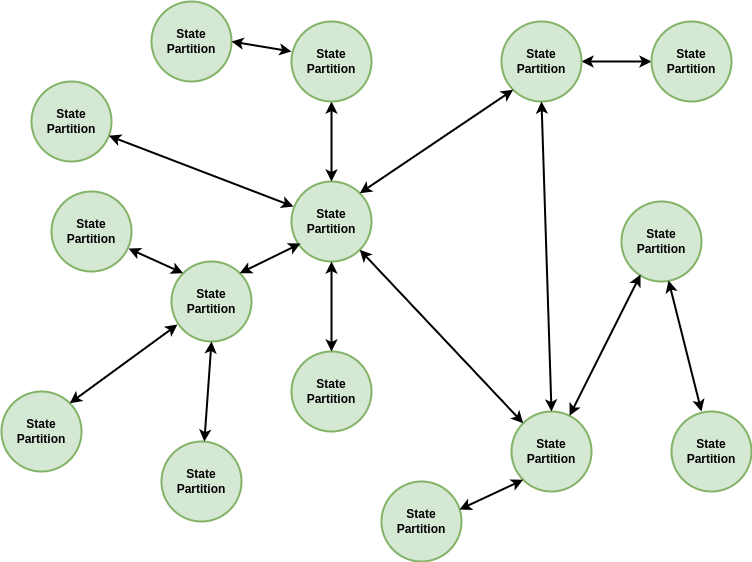
\includegraphics[width=12cm]{images/chapter-8-state-partition-graph.drawio.png}
\caption{State partition graph topology for distributed state network archetypes.}
\label{fig:state-partition-graph-distributed-state-networks}
\end{figure}

\textcolor{red}{
\begin{itemize}
\item{Talk about data}
\item{Human brain control papers}
\item{Traffic control papers}
\item{Power grid control papers}
\item{Water grid control papers} 
\end{itemize}
}
